% We-Solve contribution transcription of the supplied manuscript.
% Problem: https://we-solve.github.io/problems/complexity-of-reachability-in-the-divorce-digraph/
% Submission: https://github.com/We-Solve/research/issues/437
% Submission attribution as recorded on the GitHub issue: harisaziz.
% The substantive manuscript text, definitions, proofs, figures, algorithm,
% references and AI-assistance declaration are transcribed without rewriting.
\documentclass[11pt,letterpaper]{article}
\usepackage[T1]{fontenc}
\usepackage[utf8]{inputenc}
\usepackage{lmodern}
\usepackage[margin=1.48in]{geometry}
\usepackage{amsmath,amssymb,amsthm}
\usepackage{booktabs,array}
\usepackage{enumitem}
\usepackage{tikz}
\usetikzlibrary{positioning,arrows.meta}
\usepackage{algorithm,algpseudocode}
\usepackage{xurl}
\usepackage{titlesec}
\usepackage[unicode,hidelinks]{hyperref}
\usepackage{microtype}
\titleformat{\section}{\bfseries\normalsize}{\thesection.}{0.7em}{}
\titleformat{\subsection}{\itshape\normalsize}{\thesubsection.}{0.7em}{}
\titlespacing*{\section}{0pt}{2.0ex plus 1ex minus .2ex}{1.2ex}
\titlespacing*{\subsection}{0pt}{1.8ex plus 1ex minus .2ex}{.8ex}
\newtheorem{theorem}{Theorem}
\newtheorem{lemma}{Lemma}
\newtheorem{proposition}{Proposition}
\theoremstyle{definition}
\newtheorem{definition}{Definition}
\newtheorem{example}{Example}
\algrenewcommand\algorithmicrequire{\textbf{Input:}}
\algrenewcommand\algorithmicensure{\textbf{Output:}}
\begin{document}
\begin{center}
{\Large Divorce Reachability with Complete Preferences}
\end{center}
\vspace{1.25cm}
\hrule
\vspace{.8em}
\noindent\textbf{Abstract}
\par\noindent
A divorce matches a blocking pair and also pairs their deserted partners, preserving a perfect matching. We prove that deciding whether a stable matching is reachable by these operations is NP-hard even with strict, complete preferences. This answers the open question of whether divorce reachability remains computationally hard with complete lists. Hardness holds although every yes-instance produced by the reduction has a successful sequence of linear length. Consequently, deciding whether stability is reachable within three times the number of agents on either side is NP-complete. The unrestricted problem belongs to PSPACE, and its membership in NP remains open.

\noindent\textit{Keywords:} Stable marriage, Blocking pairs, Divorce dynamics, Reachability, Computational complexity

\noindent\textit{JEL:} C61, C78, D47
\vspace{.75em}
\hrule
\vspace{1.0em}

\section{Introduction}

Suppose every worker has a job and every position is filled, but a worker and a firm would both prefer to be matched together. One response is to revise just the two affected assignments. The worker joins the firm, and the displaced worker takes the position left vacant. Everyone remains matched, and all other assignments stay intact. Repeating this rule seems a natural way to repair an unstable assignment through small changes. Can we determine whether some choice of these changes will eventually reach stability?

The stable marriage model gives a precise setting for this question. There are two equally sized sets of agents, traditionally called men and women. Each agent strictly ranks every agent on the opposite side. A perfect matching assigns everyone one partner. A pair blocks the matching if its members prefer one another to their current partners, and a matching is stable if no pair blocks it. Gale and Shapley (1962) proved that a stable matching always exists and gave the deferred-acceptance algorithm to find one in quadratic time. When a matching already exists, we can instead ask which stable outcomes can be reached through prescribed local changes.

The rule above is Knuth's divorce operation: match a blocking pair and also match their deserted partners. It changes exactly two couples and preserves a perfect assignment. Both members of the blocking pair improve, but the deserted partners need not prefer their new assignment. This rule isolates a constrained form of local repair that keeps everyone assigned. Preferences remain fixed throughout the process. An earlier change in preferences can explain why the initial assignment is unstable.

\medskip\noindent\textit{From Knuth's question to a reachability problem.}
The question has a history going back to Knuth's 1976 monograph (Knuth, 1976), later translated into English (Knuth, 1997). Knuth showed that divorces can cycle and asked whether a suitable sequence can nevertheless bring every matching to stability, and whether a successful sequence can be short. Gusfield and Irving (1989) also highlighted the structure of the divorce relation as a possible route to finding a successful sequence.

Subsequent counterexamples revealed a stronger obstruction. Tamura (1993) and, independently, Tan and Su (1995) constructed instances with four agents on each side and starting matchings from which no divorce sequence reaches a stable matching; Tamura's construction extends to every size $n\ge 4$. A more careful choice of blocking pairs cannot rescue those starting matchings. These counterexamples turned a universal convergence question into a decision problem: distinguish the starting matchings that can reach stability from those that cannot. The question is:
\begin{quote}
Given strict, complete preferences and an initial perfect matching, can some sequence of divorces reach a stable matching?
\end{quote}
The algorithmic question remained open in the account of Manlove (2013) and the survey of Cechlárová et al. (2019, Section 3.2.2). Chen (2021) established NP-hardness for strict, incomplete lists. In Section 5, Chen singles out as the most pressing remaining question ``whether the problem remains intractable when the preferences are complete.'' Completeness is a substantive restriction here. With incomplete lists, a blocking pair may be unable to divorce because its deserted partners find one another unacceptable. With complete lists, every blocking pair permits a divorce. Removing this obstacle could, in principle, make successful paths easier to recognize. The problem is also listed in the we-solve research archive, whose record of an unverified LLM-generated attempt reports only partial results and leaves the complete-list question unresolved (we-solve research archive, 2026).

\medskip\noindent\textit{Resolving the complete-list hardness question.}
We resolve this open question by proving NP-hardness for strict, complete lists (Theorem 1). Thus, unless $\mathrm{P}=\mathrm{NP}$, there is no polynomial-time algorithm to decide whether stability is reachable even when every pair is acceptable and no agent is indifferent between partners. The difficulty lies in the permitted paths from the initial assignment, despite the polynomial-time algorithm for constructing a stable matching.

Hardness persists under a simple restriction on preferences: agents on each side have two types, every man prefers all women of his own type to all women of the other type, and every woman prefers all men of the other type to all men of her own type. The two types are equally numerous on each side. Preferences within the two blocks remain strict. The restriction provides a quantity that every divorce preserves, while the preferences inside the blocks determine which stable matchings have that quantity.

The proof separates the shape of a stable matching from the existence of a path to it. Each gadget has two possible local stable matchings. Choosing one of them represents selecting a vertex or an edge of a graph. Stability requires every selected edge to have both endpoints selected. The preserved quantity fixes the numbers of selected vertices and edges, which together encode a clique. An auxiliary gadget supplies an explicit divorce sequence for every clique. This last part is necessary: finding a stable matching with the right preserved quantity alone would not prove reachability.

Every constructed yes-instance has a successful sequence shorter than $3N$, where $N$ is the number of agents on each side. Hence the length-bounded decision problem is NP-complete even when its bound is fixed to $3N$ (Theorem 2). This also shows that the hardness of the unrestricted problem does not require long successful paths in the reduction. The result settles the complete-list hardness question. The exact complexity remains open: the polynomial-space upper bound is known, and we do not establish membership in NP for arbitrary instances.

Section 2 discusses related work. Section 3 defines the model and decision problems. Section 4 gives the reduction and its full proof. Section 5 derives the bounded-length result, and Section 6 states the remaining questions.

\section{Related work}

\noindent\textit{The divorce digraph and its history.}
Knuth introduced divorces in his monograph (Knuth, 1976, 1997). A useful way to view the process is through the divorce digraph: its vertices are perfect matchings, and an arc represents one legal divorce. With complete lists, a vertex is a sink exactly when its matching is stable. The question asks whether a designated vertex can reach any sink. Gusfield and Irving (1989) discuss the structure of this relation, and Cechlárová et al. (2019, Section 3.2.2) formulate the open decision problem in these terms. This viewpoint distinguishes a cycle encountered by one sequence from the absence of every path to stability.

Tamura (1993) and Tan and Su (1995) independently exhibit the latter phenomenon on four agents per side. Tamura also gives an algorithm that can escape a divorce cycle through an additional operation. As the survey of Cechlárová et al. (2019) explains, the running-time question for that procedure differs from divorce reachability: its output need not be connected to the initial matching by divorces alone. Our result concerns paths consisting exclusively of the original operation.

\medskip\noindent\textit{Blocking-pair dynamics with other rematching rules.}
Roth and Vande Vate (1990) show that stability is reachable from any initial matching under blocking-pair adjustment when deserted agents may remain unmatched. Their random-path result establishes almost-sure convergence in that setting. Garg and Hu (2023) give polynomial-length paths under a different set of permitted updates. These results illustrate how strongly convergence depends on the update rule. In our setting, matching the deserted partners is compulsory and every intermediate matching is perfect. A local improvement for the initiating pair can therefore create further blocking pairs through the forced new couple. The books of Gusfield and Irving (1989) and Manlove (2013) provide broader accounts of stable matching algorithms and local adjustment.

\medskip\noindent\textit{The closest complexity result and the remaining gap.}
Chen (2021) proves NP-hardness with strict, incomplete lists, even when every list has constant length. Chen also proves W[1]-hardness for the allowed number of divorces and fixed-parameter tractability when that number and the maximum list length are combined. We cite version 5 of the preprint, dated 2021, which leaves NP membership open and explicitly asks whether hardness persists with complete lists.

As in Chen's reduction, selected vertices and edges encode a clique. Complete lists require an argument that controls every available blocking pair, including those involving pairs that incomplete lists could exclude. We use a count preserved by every legal divorce to rule out successful paths on no-instances. A reservoir supplies an explicit successful path on yes-instances. Theorem 1 therefore answers the complete-list hardness question, while Theorem 2 proves NP-completeness when a linear bound on the number of divorces is imposed. Neither statement establishes NP membership for unrestricted reachability.

\section{Model and decision problems}

We first illustrate the consequence of pairing the deserted partners. Only the agents in the blocking pair must improve.

\begin{example}[A divorce can harm both deserted partners]
There are men $a,b$ and women $x,y$, with preferences
\[
\begin{aligned}
a &: y\succ x, & x &: a\succ b,\\
b &: y\succ x, & y &: a\succ b.
\end{aligned}
\]
At $\mu=\{(a,x),(b,y)\}$, pair $(a,y)$ blocks. The divorce produces $\{(a,y),(b,x)\}$, which is stable. Both $b$ and $x$ prefer their former partners, but the operation still pairs them together.
\end{example}

An instance is a tuple $I=(U,W,(\succ_z)_{z\in U\cup W})$, where $U$ is a set of $N$ men, $W$ is a disjoint set of $N$ women, and every agent has a strict total order over all agents on the opposite side. These are the usual names for the two sides of the model. All pairs are acceptable, and preferences remain fixed during the sequence. We use $u$ for a man, $w$ for a woman, and $z$ for an agent on either side.

A perfect matching $\mu$ is a set of $N$ disjoint pairs in $U\times W$. Write $\mu(z)$ for the partner of agent $z$. A pair $(u,w)\notin\mu$ is a blocking pair if
\begin{equation}\tag{1}
w\succ_u\mu(u)\qquad\text{and}\qquad u\succ_w\mu(w).
\end{equation}
A matching is stable if it has no blocking pair.

The next operation is the only permitted update. In particular, it does not leave an agent unmatched or require improvement by the deserted partners.

\begin{definition}[Divorce]
For a blocking pair $(u,w)$ of $\mu$, let $x=\mu(u)$ and $v=\mu(w)$. The divorce by $(u,w)$ produces
\begin{equation}\tag{2}
\operatorname{div}(\mu;u,w)=\bigl(\mu\setminus\{(u,x),(v,w)\}\bigr)\cup\{(u,w),(v,x)\}.
\end{equation}
\end{definition}
Completeness ensures that the result is again a feasible perfect matching. Every other couple keeps the same partners.

\begin{definition}[Reachability]
A matching $\nu$ is reachable from $\mu_0$ if there is a finite sequence $\mu_0,\ldots,\mu_t=\nu$ such that, for each $j<t$, a blocking pair $(u_j,w_j)$ of $\mu_j$ satisfies $\mu_{j+1}=\operatorname{div}(\mu_j;u_j,w_j)$. We allow $t=0$.
\end{definition}

We ask whether some sequence succeeds. Other choices of blocking pairs may cycle. The target can be any stable matching.

\begin{quote}
\noindent\textbf{DivorceSM with strict, complete lists}
\par\medskip
\noindent\begin{tabular}{@{}p{.19\linewidth}p{.74\linewidth}@{}}
\textbf{Input:}& A strict, complete stable marriage instance $I$ with $N$ agents on each side, given by explicit preference lists, and a perfect matching $\mu_0$.\\
\textbf{Question:}& Is a stable matching reachable from $\mu_0$?
\end{tabular}
\end{quote}

The bounded variant also specifies the maximum permitted number of divorces. Its encoding is part of the definition.

\begin{quote}
\noindent\textbf{Bounded DivorceSM with strict, complete lists}
\par\medskip
\noindent\begin{tabular}{@{}p{.19\linewidth}p{.74\linewidth}@{}}
\textbf{Input:}& An instance $(I,\mu_0)$ of DivorceSM and a nonnegative integer $L$ encoded in unary.\\
\textbf{Question:}& Is there a sequence of at most $L$ divorces from $\mu_0$ to a stable matching?
\end{tabular}
\end{quote}

We recall the general upper bound to distinguish the two problems. The following elementary argument is also given by Chen (2021).

\begin{proposition}
With strict, complete lists, DivorceSM belongs to PSPACE, and Bounded DivorceSM belongs to NP.
\end{proposition}
\begin{proof}
There are $N!$ perfect matchings. If a stable matching is reachable, a shortest path repeats no matching and has at most $N!-1$ divorces. A nondeterministic algorithm stores the current matching and first checks whether it is stable. If not, it guesses a blocking pair and applies its divorce. It repeats until it reaches stability or has used $N!-1$ divorces. A counter bounded by $N!$ uses $O(N\log N)$ bits. Each step uses polynomial space, so the problem belongs to nondeterministic polynomial space, which equals PSPACE.

For the bounded problem, a certificate lists at most $L$ pairs. We verify each blocking condition and update, and then check that the final matching is stable. Since $L$ is unary, the certificate and its verification have polynomial size.
\end{proof}

The $N!-1$ bound does not establish a polynomial certificate for the unrestricted problem. Our reduction will instead produce yes-instances with short paths as a property of that construction.

\section{NP-hardness with complete preferences}

This section proves that deciding the existence of a path is hard even though every man--woman pair is acceptable. The type restriction in the theorem concerns only the ordering of two blocks. It does not introduce ties.

\begin{theorem}
For strict, complete preference lists, DivorceSM is NP-hard. Hardness holds when agents have types $0$ and $1$, equally numerous on each side, every man prefers all women of his own type to all women of the other type, and every woman prefers all men of the other type to all men of her own type. Every yes-instance produced by the reduction has a successful sequence of fewer than $3N$ divorces.
\end{theorem}

Thus a polynomial-time algorithm for the complete-list problem would imply $\mathrm{P}=\mathrm{NP}$. We prove the theorem by reducing from Clique: given a simple graph $G=(V,E)$ and an integer $k$, decide whether $k$ vertices are pairwise adjacent. We restrict to $2\le k\le |V|$, which retains NP-hardness.

\subsection{The invariant and the role of the gadgets}

Under the type restriction, a divorce cannot change how many type-0 men have type-0 partners. To change that count, the initiating pair would have to make either a man or a woman move to a less preferred type. This will fix the amount that the gadgets can contribute at stability.

\begin{lemma}[Preserved count]
Suppose all men prefer their own type and all women prefer the other type. Every divorce preserves
\begin{equation}\tag{3}
q(\mu)=\bigl|\{u\in U:\operatorname{type}(u)=0,\ \operatorname{type}(\mu(u))=0\}\bigr|.
\end{equation}
\end{lemma}
\begin{proof}
If the two men have the same type, exchanging their partners preserves $q$. The same holds if the two women have the same type. Otherwise there is one man and one woman of each type. Exchanging partners either changes two same-type couples into two opposite-type couples or makes the reverse change. In the first direction neither man improves. In the reverse direction neither woman improves. Neither direction can be initiated by a blocking pair.
\end{proof}

We use a gadget with two local matchings. Its diagonal matching contributes a specified positive integer to $q$, while its cyclic matching contributes zero. At a stable matching each gadget must use one of these two choices. A vertex or edge is selected when its gadget uses the diagonal matching. Extra comparisons require selected edges to have selected endpoints. A large auxiliary gadget, called the reservoir, initially holds the entire preserved count and later transfers it to the selected gadgets.

\begin{table}[htbp]
\centering
\begin{tabular}{@{}lcc@{}}
\toprule
Gadget $g$ & Weight $s_g$ & Number of agents on each side\\
\midrule
Vertex $v\in V$ & $1$ & $2$\\
Edge $e\in E$ & $B$ & $2B$\\
Reservoir $R$ & $T+1$ & $2(T+1)$\\
\bottomrule
\end{tabular}
\caption{The gadgets in the reduction. The diagonal matching of gadget $g$ contributes $s_g$ to the preserved count $q$. Its cyclic matching contributes zero.}
\end{table}

\subsection{Agents and complete preference lists}

Fix a Clique instance $(G,k)$, and write $n=|V|$. Define
\begin{equation}\tag{4}
B=n+1,\qquad T=k+B\binom{k}{2}.
\end{equation}
The multiplier $B$ will separate the number of selected vertices from the number of selected edges. The target count is $T$.

Create one gadget for each vertex, one for each edge, and the reservoir $R$. A gadget $g$ has weight $s_g$ as specified in Table 1 and contains men $u_{g,i}$ and women $w_{g,i}$ for $i=0,\ldots,2s_g-1$. Both agents with index $i$ have type $i\bmod 2$. Indices within each gadget are interpreted modulo $2s_g$.

The two local matchings are
\begin{equation}\tag{5}
D_g=\{(u_{g,i},w_{g,i}):0\le i<2s_g\},\quad C_g=\{(u_{g,i},w_{g,i+1}):0\le i<2s_g\}.
\end{equation}
We call them the \textbf{diagonal} and \textbf{cyclic} matchings.

Every man $u_{g,i}$ has the following preference blocks, from best to worst:
\begin{enumerate}[label=(\roman*),leftmargin=2.7em,itemsep=.45ex]
\item his own woman $w_{g,i}$;
\item all other women of his own type;
\item his cyclic successor $w_{g,i+1}$;
\item all remaining women of the opposite type.
\end{enumerate}
For a reservoir man, block (iv) lists all remaining opposite-type reservoir women before all opposite-type women outside the reservoir. This refinement will make the second phase of a transfer legal.

For a woman $w_{g,i}$, let $H_{g,i}$ contain the following distinguished same-type men:
\begin{equation}\tag{6}
H_{g,i}=\begin{cases}
\{u_{v,0},u_{v',0}\},&g=\{v,v'\}\in E,\ i=0,\\
\{u_{h,j}:h\in V\cup E,\ j\equiv i\pmod{2}\},&g=R,\\
\varnothing,&\text{otherwise.}
\end{cases}
\end{equation}
Here the sets range over agents created above. The comparisons at an edge gadget will enforce its incidence conditions. The comparisons at the reservoir will allow any original gadget to receive the required count.

Every woman $w_{g,i}$ ranks:
\begin{enumerate}[label=(\roman*),leftmargin=2.7em,itemsep=.6ex]
\item her cyclic predecessor $u_{g,i-1}$;
\item all other men of the opposite type;
\item the men in $H_{g,i}$;
\item her own man $u_{g,i}$;
\item all remaining men of her own type.
\end{enumerate}
Fix arbitrary strict orders inside every remaining block. Each agent on the opposite side appears exactly once, so these are complete, strict lists. The proof works for every such completion satisfying the stated reservoir refinement.

Initially, every vertex and edge gadget uses its cyclic matching. The reservoir uses diagonal pairs at indices $0,\ldots,2T-1$, and its remaining two men exchange their women. Formally,
\begin{equation}\tag{7}
\begin{aligned}
\mu_0={}&\bigcup_{g\in V\cup E} C_g\ \cup\ \{(u_{R,i},w_{R,i}):0\le i<2T\}\\
&\cup\ \{(u_{R,2T},w_{R,2T+1}),(u_{R,2T+1},w_{R,2T})\}.
\end{aligned}
\end{equation}
This is perfect, and
\begin{equation}\tag{8}
q(\mu_0)=T.
\end{equation}
There are equally many agents of each type on each side. The total number on each side is
\begin{equation}\tag{9}
N=2n+2B|E|+2(T+1)=O(n^3).
\end{equation}
The complete lists therefore have polynomial input length and can be written in polynomial time. The weights are implemented by agents, not by succinctly encoded multiplicities.

\subsection{The stable matchings of the construction}

We next account for every stable matching, including potential pairs between gadgets. Two first-choice arguments restrict such pairs. Balance then excludes them.

\begin{lemma}[Local form at stability]
In every stable matching of the constructed instance, every gadget is matched internally and uses either $D_g$ or $C_g$.
\end{lemma}
\begin{proof}
Fix a stable matching $\mu$. If man $u_{g,i}$ has an opposite-type partner other than $w_{g,i+1}$, then he prefers $w_{g,i+1}$ to that partner. Woman $w_{g,i+1}$ ranks him first overall, so they block. Thus an opposite-type stable partner of $u_{g,i}$ must be his cyclic successor.

If woman $w_{g,i}$ has a same-type partner outside $H_{g,i}\cup\{u_{g,i}\}$, then she prefers her own man to that partner. Her own man ranks her first overall, so they block. Hence a same-type stable pair is either diagonal or uses a man in $H_{g,i}$.

It follows from (6) that every pair between different gadgets has a man in a vertex gadget and a woman in an incident edge gadget, or has a man in a vertex or edge gadget and a woman in the reservoir. Contract each gadget to one vertex and direct each such pair from its man's gadget to its woman's gadget. This is a directed multigraph whose arcs follow the acyclic order
\[
\text{vertex gadgets},\qquad\text{edge gadgets},\qquad R.
\]
Each gadget has equally many men and women. Subtracting its internal pairs shows that its outdegree equals its indegree. A finite acyclic directed multigraph with balanced degrees has no arcs: a source has indegree zero and hence outdegree zero, and we repeat after removing it. Thus no stable pair joins different gadgets.

Within gadget $g$, the only remaining possible pairs are diagonal pairs and cyclic-successor pairs. If one man receives his successor, that woman is unavailable to her own man, who must also receive his successor. Continuing around the gadget forces $C_g$. If no man receives his successor, all pairs are diagonal and the matching is $D_g$.
\end{proof}

The argument also shows that stable matchings exist independently of the input graph. Putting every gadget in its diagonal matching gives every man his first choice. Putting every gadget in its cyclic matching gives every woman her first choice. The question is which stable matchings the initial count permits.

\begin{example}[A four-by-four obstruction]
Consider an isolated weight-two gadget with the same preference blocks and all distinguished sets empty. Its only stable matchings are $D_g$ and $C_g$, by the local argument in Lemma 2. Their counts are $2$ and $0$. The matching with diagonal pairs at indices $0,1$ and crossed pairs at indices $2,3$ has count $1$. Lemma 1 therefore excludes every path to stability. This illustrates the obstruction used by the reduction without a search of the divorce graph. Tamura's own four-by-four example, as reproduced by Chen (2021, Example 2), also satisfies the two-type restriction. Its starting matching has count $1$, while every stable matching has count $0$ or $2$, so Lemma 1 also explains why no divorce sequence succeeds there.
\end{example}

A reachable stable matching cannot use the reservoir's diagonal matching, because that would contribute too much to the count. Once the reservoir is cyclic, the remaining stability conditions express exactly the graph's incidences.

\begin{lemma}[Selected edges require their endpoints]
Consider a matching in which every gadget uses $D_g$ or $C_g$ and the reservoir uses $C_R$. This matching is stable if and only if every edge gadget using $D_e$ has both endpoint gadgets using their diagonal matchings.
\end{lemma}
\begin{proof}
A man in $D_g$ receives his first choice and belongs to no blocking pair. A man in $C_g$ receives his best opposite-type woman, so he can block only with a same-type woman. A woman in $C_g$ receives her first choice and belongs to no blocking pair. A woman in $D_g$ prefers another same-type man to her partner exactly when that man belongs to $H_{g,i}$.

All reservoir women receive their first choices in $C_R$. At a vertex or edge gadget, the only nonempty distinguished sets are $H_{e,0}$ for edges $e=\{v,v'\}$. The possible blocking pairs are therefore $(u_{v,0},w_{e,0})$ and $(u_{v',0},w_{e,0})$. The first blocks exactly when $v$ is cyclic and $e$ is diagonal, and the second has the corresponding condition for $v'$. This proves both directions.
\end{proof}

\subsection{Soundness: every successful path identifies a clique}

The invariant now turns the stability conditions into exact counts of vertices and edges. This part of the proof applies to paths of any length and allows every legal choice of blocking pair.

\begin{lemma}
If a stable matching is reachable from $\mu_0$, then $G$ has a $k$-clique.
\end{lemma}
\begin{proof}
Let $\mu$ be a reachable stable matching. By Lemma 1 and (8), $q(\mu)=T$. Lemma 2 gives the two local choices at every gadget. The reservoir must use $C_R$, since $D_R$ alone contributes $T+1>T$.

Select a vertex or edge when its gadget is diagonal. Let $a$ count the selected vertices and $b$ the selected edges. Their contributions give
\begin{equation}\tag{10}
a+Bb=T=k+B\binom{k}{2}.
\end{equation}
Both $a$ and $k$ lie between $0$ and $n<B$. Reduction modulo $B$ therefore gives $a=k$, and then (10) gives $b=\binom{k}{2}$.

By Lemma 3, every selected edge has both endpoints among the $k$ selected vertices. A simple graph has at most $\binom{k}{2}$ edges on those vertices. Since that many distinct edges are selected, the vertices form a clique.
\end{proof}

\subsection{Completeness: transferring the count by legal divorces}

We must also construct a path when a clique exists. The invariant is only a necessary condition for arbitrary starting matchings, so we do not infer reachability from a stable matching with count $T$. Instead, the reservoir permits a direct transfer into any chosen gadget. Figure 1 illustrates a weight-one transfer.

\begin{figure}[htbp]
\centering
\small
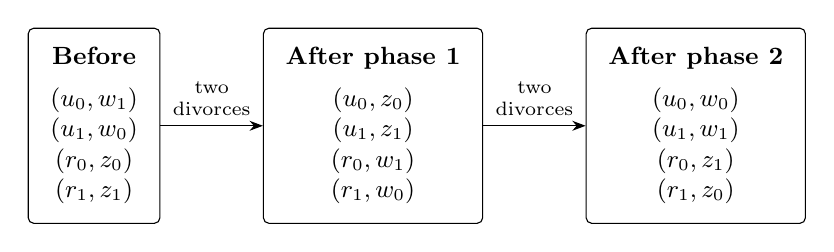
\begin{tikzpicture}[
  >=Stealth,
  box/.style={draw,rounded corners=2pt,inner xsep=8pt,inner ysep=7pt,align=center},
  every node/.style={font=\small}
]
\node[box] (before) {\textbf{Before}\\[4pt]
$(u_0,w_1)$\\$(u_1,w_0)$\\$(r_0,z_0)$\\$(r_1,z_1)$};
\node[box,right=1.3cm of before] (one) {\textbf{After phase 1}\\[4pt]
$(u_0,z_0)$\\$(u_1,z_1)$\\$(r_0,w_1)$\\$(r_1,w_0)$};
\node[box,right=1.3cm of one] (two) {\textbf{After phase 2}\\[4pt]
$(u_0,w_0)$\\$(u_1,w_1)$\\$(r_0,z_1)$\\$(r_1,z_0)$};
\draw[->] (before) -- node[above,align=center,font=\scriptsize]{two\\divorces} (one);
\draw[->] (one) -- node[above,align=center,font=\scriptsize]{two\\divorces} (two);
\end{tikzpicture}
\caption{A transfer into a weight-one gadget. The original agents are $u_0,u_1,w_0,w_1$. The initially diagonal reservoir couples are $(r_0,z_0)$ and $(r_1,z_1)$, with index giving the type. Phase 1 uses blocking pairs $(u_i,z_i)$. Phase 2 uses $(r_i,z_{i+1})$, with indices modulo two. The gadget gains one unit of $q$, and the reservoir loses one. Each arrow denotes two separate legal divorces.}
\end{figure}

\begin{lemma}[Transfer]
Suppose a vertex or edge gadget $g$ uses $C_g$. Given $s_g$ unused diagonal reservoir couples of each type, $4s_g$ legal divorces put $g$ into $D_g$ and turn all those reservoir couples into opposite-type reservoir couples. No other agents change partners.
\end{lemma}
\begin{proof}
Suppress $g$ in the notation and put $s=s_g$. Choose distinct diagonal reservoir couples $(r_i,z_i)$ for $0\le i<2s$, with both agents of type $i\bmod 2$. These are unused, so each consists of a reservoir man and his own woman. Interpret the local indices in this proof modulo $2s$.

\noindent\textit{Phase 1: bring each original man to a reservoir woman.}
For every $i$, use blocking pair $(u_i,z_i)$ to perform
\begin{equation}\tag{11}
\{(u_i,w_{i+1}),(r_i,z_i)\}\longrightarrow\{(u_i,z_i),(r_i,w_{i+1})\}.
\end{equation}
Man $u_i$ improves from an opposite-type woman to a same-type woman. Woman $z_i$ prefers every original same-type man to her own man, by her distinguished set in (6). Thus the initiating pair blocks. The $2s$ operations use disjoint sets of agents, so earlier operations do not change the premises for later ones.

\noindent\textit{Phase 2: return the original men to their own women.}
After all phase-1 operations, use $(r_i,z_{i+1})$ for each $i$:
\begin{equation}\tag{12}
\{(r_i,w_{i+1}),(u_{i+1},z_{i+1})\}\longrightarrow\{(r_i,z_{i+1}),(u_{i+1},w_{i+1})\}.
\end{equation}
The two possible partners of $r_i$ in this display both have the opposite type. Woman $w_{i+1}$ lies outside the reservoir, so she is not the cyclic successor of $r_i$ and appears in the non-reservoir part of his block (iv). Woman $z_{i+1}$ is either his cyclic successor, in block (iii), or a reservoir woman in block (iv). By the reservoir refinement, $r_i$ ranks $z_{i+1}$ above $w_{i+1}$ in both cases. Woman $z_{i+1}$ improves from the same-type man $u_{i+1}$ to the opposite-type man $r_i$. Hence this pair blocks too. These $2s$ operations again use disjoint sets of agents.

Every original man now has his own woman. The chosen reservoir men are matched to the next chosen reservoir women, whose types are opposite because the cycle has even length. The two phases use $4s$ divorces and affect no other agents.
\end{proof}

We apply these transfers to the gadgets selected by a clique. Once all diagonal reservoir couples have been used, only the reservoir may need further adjustment. Since all its couples are then opposite-type couples, we can give each reservoir woman her first choice using further legal divorces.

Algorithm 1 specifies the path. An unused reservoir couple means one of the initial diagonal couples not assigned to a previous transfer. Fix an order of the graph's vertices and edges and of all agents. All selections in the algorithm use that order. The operation Apply replaces $\mu$ by $\operatorname{div}(\mu;u,w)$ and appends the initiating pair $(u,w)$ to the output sequence.

\begin{lemma}[A short path from a clique]
If $G$ has a $k$-clique, Algorithm 1 returns a successful sequence of at most $6T+2<3N$ divorces. The sequence can be constructed and checked in polynomial time.
\end{lemma}

\begin{algorithm}[!t]
\caption{A successful divorce sequence from a clique}
\begin{algorithmic}[1]
\Require Constructed instance $(I,\mu_0)$ and a $k$-clique $S$ of $G$.
\Ensure A sequence of fewer than $3N$ legal divorces ending at stability.
\State $\mu\gets\mu_0$; initialize the output sequence to empty.
\State Select the vertex gadgets of $S$ and the edge gadgets within $S$.
\For{each selected gadget $g$ in the fixed order}
\State Choose the first $s_g$ unused diagonal reservoir couples of each type.
\State Label them $(r_i,z_i)$ for $0\le i<2s_g$, preserving types.
\For{$i=0,\ldots,2s_g-1$}
\State Apply$(u_{g,i},z_i)$.
\EndFor
\For{$i=0,\ldots,2s_g-1$}
\State Apply$(r_i,z_{i+1})$, with indices modulo $2s_g$.
\EndFor
\State Mark the chosen reservoir couples as used.
\EndFor
\For{$i=0,\ldots,2T+1$}
\If{$\mu(u_{R,i})\ne w_{R,i+1}$}
\State Apply$(u_{R,i},w_{R,i+1})$, modulo $2T+2$.
\EndIf
\EndFor
\State \Return the output sequence.
\end{algorithmic}
\end{algorithm}
\begin{proof}
Select the $k$ vertex gadgets of the clique and all its $\binom{k}{2}$ edge gadgets. By (4), their total weight is $T$. The reservoir initially has $T$ diagonal couples of each type. Each transfer needs exactly its gadget's weight of each type, and previously used couples are never chosen again. There are therefore enough unused couples for every transfer.

Lemma 5 proves the legality of both transfer loops. Each selected gadget becomes diagonal and every other original gadget stays cyclic. The transfers use $4\sum_{g\text{ selected}}s_g=4T$ divorces. Since the selected weights sum to exactly $T$, the transfers use all $2T$ initial diagonal reservoir couples, and each becomes an opposite-type reservoir couple. The two couples at indices $2T$ and $2T+1$ were opposite-type from the start and are untouched by the transfers. Hence all reservoir couples are now opposite-type couples within the reservoir.

Consider a reservoir man not paired with his cyclic successor. He ranks her first among opposite-type women, and she ranks him first overall. Since his current partner is another opposite-type reservoir woman, the pair blocks. Its divorce keeps both resulting reservoir couples opposite-type. It also leaves every already correct cyclic pair intact: neither member of a correct pair can be a deserted partner in a divorce by a different cyclic pair. The final loop thus produces $C_R$ in at most $2(T+1)$ operations.

Every selected edge has both endpoints selected. The final matching is stable by Lemma 3. The total length is at most $4T+2(T+1)=6T+2$.

Finally, (9) gives
\[
3N=6n+6B|E|+6T+6>6T+2.
\]
The instance has polynomial size, each operation can be carried out in polynomial time, and there are $O(T)$ operations. This proves the running-time assertion.
\end{proof}



\noindent\textit{Proof of Theorem 1.}
The construction is polynomial by (9) and satisfies all preference and type restrictions in the theorem. Lemma 4 proves that every successful path gives a $k$-clique. Lemma 6 constructs a path from every $k$-clique, with the stated length bound. Thus the construction is a polynomial-time many-one reduction from Clique to DivorceSM.

The soundness argument uses the invariant for arbitrary paths. The completeness argument supplies a particular path and checks both members of every initiating pair. All other legal moves remain available throughout. No part of the proof requires the dynamic to choose the constructed sequence unless we are establishing that some successful sequence exists.

\section{Hardness with a linear divorce bound}

The same construction answers a stronger bounded question. It is hard to recognize a short path even when the permitted length is fixed as a linear function of the market size.

\begin{theorem}
With strict, complete preference lists, Bounded DivorceSM is NP-complete, even when its bound is fixed to $L=3N$ and preferences satisfy the two-type restrictions of Theorem 1.
\end{theorem}
\begin{proof}
Membership in NP is Proposition 1. For hardness, construct $(I,\mu_0)$ from $(G,k)$ as above and set $L=3N$. The unary encoding of $L$ has polynomial size. If the graph has a $k$-clique, Lemma 6 gives a successful path shorter than $L$. If it has no $k$-clique, Lemma 4 excludes a successful path of any length. The reduction therefore also proves NP-hardness with this fixed linear bound.
\end{proof}

This result does not assert that every reachable stable matching in an arbitrary complete instance has a short witness. The linear bound is guaranteed for the yes-instances produced by the reduction. That distinction is why Theorem 2 is an NP-completeness statement while Theorem 1 is an NP-hardness statement.

\section{Conclusion}

We resolve the open question of whether divorce reachability remains computationally hard with strict, complete preferences. Theorem 1 proves NP-hardness, answering the complete-list question left open by Chen (2021) in the line of work originating with Knuth. The hardness holds even though a linear-length successful path suffices on every constructed yes-instance. Imposing the fixed bound $3N$ yields NP-completeness.

The main remaining question is the exact complexity of unrestricted DivorceSM. Does every yes-instance with complete lists have a polynomial-size certificate, perhaps a polynomial-length divorce sequence? Alternatively, can the polynomial-space upper bound be matched by a PSPACE-hardness reduction? The present construction does not distinguish these possibilities.

The invariant also suggests a structural question. Which restrictions on preferences ensure that a stable matching with a given preserved count is reachable from a given starting matching? Our reservoir establishes this implication for the particular starting matchings used in the reduction. A general condition would help identify tractable domains of divorce reachability.

Tamura's procedure, which permits an additional operation when divorces cycle, has a different termination-time question. The hardness result for pure divorces does not determine the running time of that procedure.

\section*{Declaration of generative AI assistance}

OpenAI's ChatGPT assisted with developing the reduction and preparing the manuscript.

\section*{References}
\begin{list}{}{\setlength{\leftmargin}{1em}\setlength{\itemindent}{-1em}\setlength{\itemsep}{.75em}\setlength{\parsep}{0pt}}
\item K. Cechlárová, Á. Cseh, and D. F. Manlove. Selected open problems in matching under preferences. \emph{Bulletin of the European Association for Theoretical Computer Science}, (128), 2019. URL \url{https://bulletin.eatcs.org/index.php/beatcs/article/view/586}. (Cited on pp. 2 and 4.)

\item J. Chen. Reaching stable marriage via divorces is hard, 2021. URL \url{https://arxiv.org/abs/1906.12274v5}. arXiv:1906.12274v5. First posted in 2019. (Cited on pp. 2, 4, 6, 11, and 16.)

\item D. Gale and L. S. Shapley. College admissions and the stability of marriage. \emph{The American Mathematical Monthly}, 69(1):9--15, 1962. doi: 10.1080/00029890.1962.11989827. (Cited on p. 1.)

\item V. K. Garg and C. Hu. Improved paths to stability for the stable marriage problem. In \emph{Proceedings of the 25th International Symposium on Stabilization, Safety, and Security of Distributed Systems (SSS)}, volume 14310 of \emph{Lecture Notes in Computer Science}, pages 126--140. Springer, 2023. doi: 10.1007/978-3-031-44274-2\_11. (Cited on p. 4.)

\item D. Gusfield and R. W. Irving. \emph{The Stable Marriage Problem: Structure and Algorithms}. MIT Press, 1989. (Cited on pp. 2 and 4.)

\item D. E. Knuth. \emph{Mariages stables et leurs relations avec d'autres problèmes combinatoires}. Les Presses de l'Université de Montréal, 1976. (Cited on pp. 2 and 3.)

\item D. E. Knuth. \emph{Stable Marriage and Its Relation to Other Combinatorial Problems: An Introduction to the Mathematical Analysis of Algorithms}, volume 10 of CRM Proceedings and Lecture Notes. American Mathematical Society, 1997. (Cited on pp. 2 and 3.)

\item D. F. Manlove. \emph{Algorithmics of Matching Under Preferences}, volume 2 of \emph{Series on Theoretical Computer Science}. World Scientific, 2013. (Cited on pp. 2 and 4.)

\item A. E. Roth and J. H. Vande Vate. Random paths to stability in two-sided matching. \emph{Econometrica}, 58(6):1475--1480, 1990. doi: 10.2307/2938326. (Cited on p. 4.)

\item A. Tamura. Transformation from arbitrary matchings to stable matchings. \emph{Journal of Combinatorial Theory, Series A}, 62(2):310--323, 1993. doi: 10.1016/0097-3165(93)90051-9. (Cited on pp. 2 and 4.)

\item J. J. M. Tan and W. C. Su. On the divorce digraph of the stable marriage problem. \emph{Proceedings of the National Science Council, Republic of China, Part A}, 19(2):342--354, 1995. (Cited on pp. 2 and 4.)

\item we-solve research archive. GPT 6 Astra Ultra attempt on Econ-139 (ECON-C78-136). \url{https://we-solve.github.io/contributions/complexity-of-reachability-in-the-divorce-digraph/attempt-1/r1/}, October 2026. Revision r1 of ECON-C78-136-A1. Unverified research record. LLMs and submitter roles are disclosed in the record. (Cited on p. 2.)
\end{list}
\end{document}
